\documentclass[11pt,letterpaper]{article}
\usepackage[utf8]{inputenc}
\usepackage[T1]{fontenc}
\usepackage{lmodern}
\usepackage[margin=2.54cm,top=1.78cm,bottom=1.78cm]{geometry}
\usepackage{graphicx,longtable,array,hyperref,listings}
\pdfimageresolution=72
\urlstyle{same}
\hypersetup{hidelinks,pdftitle={Informe Laboratorio 3 - 2026},pdfauthor={Francisco Antonio Tapia Canales},pdfsubject={Criptografía y Seguridad en Redes CIT2113},pdflang={es-CL}}
\lstset{basicstyle=\ttfamily\footnotesize,breaklines=true,columns=fullflexible,literate={ñ}{{\~n}}1}
\setlength{\parindent}{0pt}
\setlength{\parskip}{6pt}
\renewcommand{\contentsname}{Índice}
\begin{document}
\raggedright
\begin{center}{\LARGE Informe Laboratorio 3}\end{center}
\begin{center}Sección 2\\[9pt]
Francisco Antonio Tapia Canales\\
e-mail: \href{mailto:francisco.tapia1@mail.udp.cl}{francisco.tapia1@mail.udp.cl}\\[9pt]
Criptografía y Seguridad en Redes CIT2113\\
Profesor René Guerrero\\
Octubre de 2026\end{center}
\tableofcontents
\newpage
\section*{1. Descripción de actividades}
\addcontentsline{toc}{section}{1. Descripción de actividades}
El objetivo de este laboratorio fue auditar la transformación de contraseñas en páginas web desde el lado del cliente y evaluar la reutilización de un hash para iniciar sesión, según la prueba Pass the Hash solicitada en la pauta.\par
Seleccioné \url{https://www.forodvd.com/} y creé una cuenta propia de prueba con una contraseña destinada a esta actividad. Trabajé con Ubuntu en VMware Workstation y con el navegador integrado de Burp Suite Community.\par
Realicé las siguientes actividades:\par
$\bullet$ Identifiqué el algoritmo hash utilizado al registrar la cuenta.\par
$\bullet$ Comparé los parámetros enviados durante el inicio de sesión.\par
$\bullet$ Calculé el hash de la contraseña desde la consola del navegador.\par
$\bullet$ Detuve una solicitud de login en Proxy Intercept de Burp Suite.\par
$\bullet$ Probé el rechazo de una contraseña incorrecta y repetí el acceso sustituyendo sus hashes por el valor correcto.\par
$\bullet$ Revisé la política de privacidad enlazada por el sitio y los controles observados en la interfaz.\par
$\bullet$ Elaboré cuatro conclusiones sobre los resultados y su alcance.\par
La práctica mostró que el registro y el login enviaron MD5 en el cliente. La contraseña incorrecta fue rechazada, mientras que la solicitud con el hash correcto reutilizado abrió una sesión. La cuenta mantuvo pendiente la activación por correo para participar en el foro.\par
Al concluir envié un cambio de contraseña y conservé la confirmación de actualización del perfil. La contraseña nueva no forma parte de las evidencias.\par
\newpage
\section*{2. Desarrollo de actividades según criterio de rúbrica}
\addcontentsline{toc}{section}{2. Desarrollo de actividades según criterio de rúbrica}
\subsection*{2.1. Identifica el algoritmo hash utilizado para las contraseñas al momento del registro en el sitio web}
\addcontentsline{toc}{subsection}{2.1. Identifica el algoritmo hash utilizado para las contraseñas al momento del registro en el sitio web}
Después de registrar la cuenta, identifiqué en Burp la solicitud POST a \nolinkurl{/register.php?do=addmember}. Los parámetros \nolinkurl{password_md5} y \nolinkurl{passwordconfirm_md5} contenían el mismo valor. Los campos password y passwordconfirm aparecían vacíos.\par
\begin{lstlisting}
password_md5 = 95e5ffce381c006ca63266ecc0ac6771
passwordconfirm_md5 = 95e5ffce381c006ca63266ecc0ac6771
\end{lstlisting}
Identifiqué MD5 mediante la biblioteca pública \nolinkurl{vbulletin_md5}.js y la coincidencia con \nolinkurl{hex_md5} al ingresar la misma contraseña en la consola. El tamaño de 32 caracteres hexadecimales es compatible con MD5, pero la identificación también se apoyó en el código y en esa comparación. [S1-S2]\par
\begin{center}\begin{minipage}{\linewidth}\centering
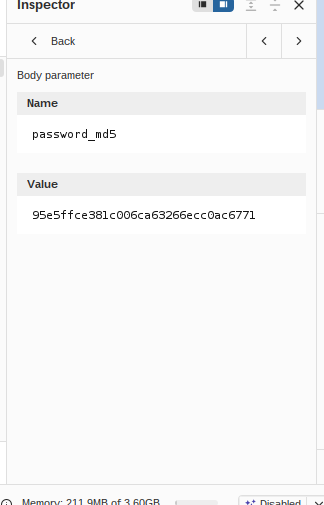
\includegraphics[width=2.8in,trim=7.5010bp 195.0272bp 10.5015bp 63.7589bp,clip]{evidencias/E01_registro_md5.png}
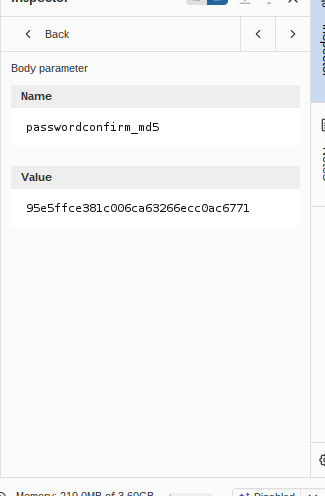
\includegraphics[width=2.8in,trim=7.5010bp 195.7773bp 11.2516bp 60.0084bp,clip]{evidencias/E01_registro_confirmacion.png}
\par\smallskip
{\small Figura 1. Campos password\_md5 y passwordconfirm\_md5 del registro.}
\end{minipage}\end{center}
\subsection*{2.2. Identifica el algoritmo hash utilizado para las contraseñas al momento de iniciar sesión}
\addcontentsline{toc}{subsection}{2.2. Identifica el algoritmo hash utilizado para las contraseñas al momento de iniciar sesión}
La solicitud POST a \nolinkurl{/login.php?do=login} envió el mismo valor en \nolinkurl{vb_login_md5password} y \nolinkurl{vb_login_md5password_utf}. El parámetro \nolinkurl{vb_login_password} quedó vacío. Para la contraseña utilizada, los dos campos coincidieron con el registro y con la consola.\par
El formulario público ejecuta md5hash al enviarse y carga la biblioteca que define \nolinkurl{hex_md5}. Esto permite ubicar la transformación en el navegador. Las capturas describen el valor enviado por el cliente; el almacenamiento interno del servidor no se observó. [S1-S2]\par
\begin{center}\begin{minipage}{\linewidth}\centering
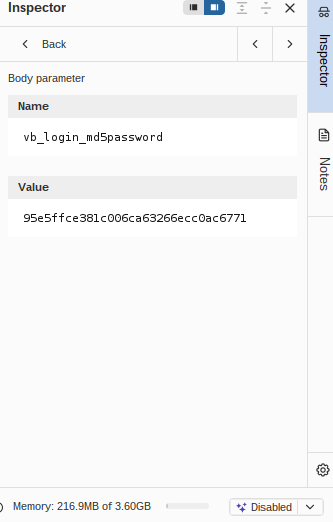
\includegraphics[width=2.8in,trim=7.5010bp 204.0285bp 17.2524bp 67.5094bp,clip]{evidencias/E02_login_md5.png}
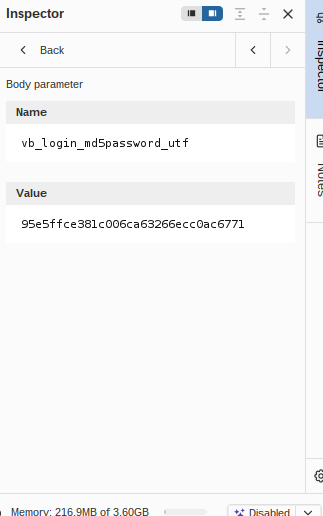
\includegraphics[width=2.8in,trim=7.5010bp 195.7773bp 9.7514bp 71.2599bp,clip]{evidencias/E02_login_md5_utf.png}
\par\smallskip
{\small Figura 2. Ambos campos de login contienen el mismo MD5 que el registro.}
\end{minipage}\end{center}
\newpage
\section*{2.3. Genera el hash de la contraseña desde la consola del navegador}
\addcontentsline{toc}{subsection}{2.3. Genera el hash de la contraseña desde la consola del navegador}
En la consola del navegador de ForoDVD ejecuté la función disponible en la página. Escribí la contraseña de prueba en el cuadro de diálogo generado por prompt.\par
\begin{lstlisting}
hex_md5(prompt("Introduce la contraseña que usaste al registrarte"))
\end{lstlisting}
\begin{center}\begin{minipage}{\linewidth}\centering
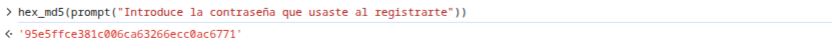
\includegraphics[width=6.5in]{evidencias/E03_consola.png}
\par\smallskip
{\small Figura 3. Recorte de la captura original con el comando correcto y su resultado.}
\end{minipage}\end{center}
El resultado fue 95e5ffce381c006ca63266ecc0ac6771. Coincidió con \nolinkurl{password_md5} del registro y con los dos parámetros MD5 del login. Ingresé la contraseña en el cuadro de diálogo de prompt; la función \nolinkurl{hex_md5} ya estaba cargada por ForoDVD. [S2]\par
\subsection*{2.4. Intercepta el tráfico login con Burp Suite}
\addcontentsline{toc}{subsection}{2.4. Intercepta el tráfico login con Burp Suite}
En Burp abrí Proxy, utilicé Open browser y navegué hasta el formulario de acceso. Activé Intercept antes de pulsar Iniciar sesión y seleccioné la petición POST a \nolinkurl{/login.php?do=login}. La figura 4 muestra Intercept on y la solicitud detenida. [S4]\par
\begin{center}\begin{minipage}{\linewidth}\centering
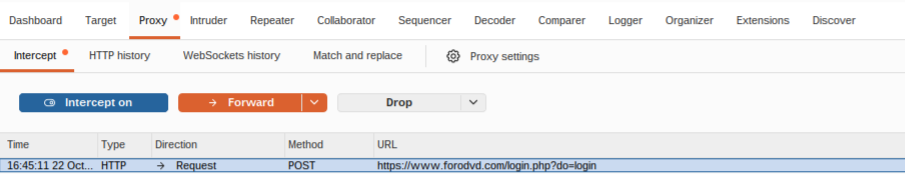
\includegraphics[width=6.5in]{evidencias/E04_intercept.png}
\par\smallskip
{\small Figura 4. Petición POST de login detenida en Proxy Intercept.}
\end{minipage}\end{center}
Revisé los campos en Inspector y después en Raw. En la captura de la figura 5, correspondiente al intento con contraseña incorrecta, \nolinkurl{vb_login_md5password} contenía el valor indicado. Ambos campos se modificaron en el punto 2.5. [S5]\par
\begin{center}\begin{minipage}{\linewidth}\centering
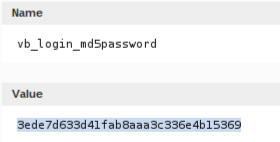
\includegraphics[width=3.1in]{evidencias/E04_hash_incorrecto.png}
\par\smallskip
{\small Figura 5. Hash de la contraseña incorrecta observado en la solicitud detenida.}
\end{minipage}\end{center}
La captura se realizó desde el navegador configurado con Burp. Este resultado acredita la inspección de esa sesión, sin demostrar una interceptación de HTTPS desde un equipo ajeno al navegador de prueba.\par
\newpage
\section*{2.5. Realizar el intento de login por medio del hash}
\addcontentsline{toc}{subsection}{2.5. Realizar el intento de login por medio del hash}
Primero comprobé el acceso normal y cerré la sesión. Después envié una contraseña incorrecta, sin sustituir sus hashes, para observar el comportamiento de rechazo.\par
El hash correcto se había observado en los campos del login capturado en Burp (figura 2) y se comprobó con la consola (figura 3).\par
{\small\renewcommand{\arraystretch}{1.12}
\begin{longtable}{|>{\raggedright\arraybackslash}p{3.03cm}|>{\raggedright\arraybackslash}p{8.73cm}|>{\raggedright\arraybackslash}p{3.37cm}|}
\hline
\textbf{Prueba} & \textbf{Credencial enviada} & \textbf{Resultado}\\\hline
\endhead
A Control correcto & Hash generado a partir de la contraseña correcta. & Sesión iniciada.\\\hline
B Control incorrecto & Hash generado a partir de una contraseña incorrecta. & Acceso rechazado.\\\hline
C Sustitución & Contraseña incorrecta en el formulario y ambos hashes reemplazados por el correcto. & Sesión iniciada.\\\hline
\end{longtable}
}
\begin{center}\begin{minipage}{\linewidth}\centering
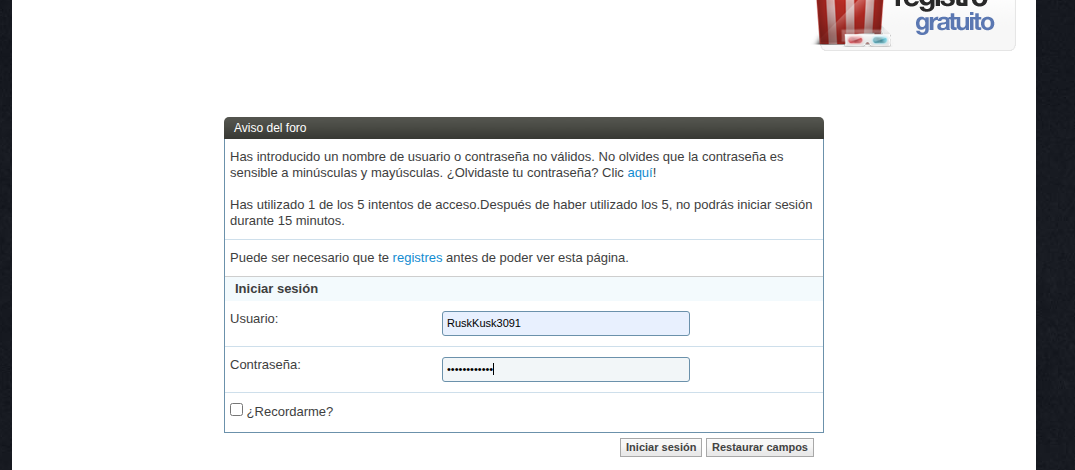
\includegraphics[width=6.5in,trim=168.0235bp 170.2738bp 187.5262bp 87.0121bp,clip]{evidencias/E06_control_login_incorrecto.png}
\par\smallskip
{\small Figura 6. Rechazo del acceso con contraseña incorrecta antes de sustituir el hash.}
\end{minipage}\end{center}
El sitio informó un intento utilizado de cinco e indicó un bloqueo de 15 minutos al agotar ese límite. La captura acredita el aviso; no agoté los intentos para comprobar el bloqueo.\par
Repetí el ingreso con una contraseña incorrecta y activé Intercept antes de enviar. Ambos parámetros contenían el hash incorrecto indicado abajo. En Raw sustituí únicamente esos dos valores por el hash correcto, conservando los demás datos de la solicitud vigente.\par
\begin{lstlisting}
Hash incorrecto observado:
3ede7d633d41fab8aaa3c336e4b15369

Hash correcto reutilizado:
95e5ffce381c006ca63266ecc0ac6771
\end{lstlisting}
\begin{center}\begin{minipage}{\linewidth}\centering
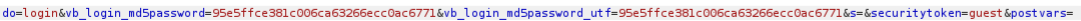
\includegraphics[width=6.5in,trim=0.0000bp 0.0000bp 636.1449bp 0.0000bp,clip]{evidencias/E07_solicitud_modificada.png}
\\
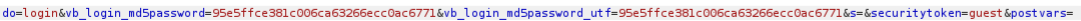
\includegraphics[width=6.5in,trim=435.0991bp 0.0000bp 231.0526bp 0.0000bp,clip]{evidencias/E07_solicitud_modificada.png}
\par\smallskip
{\small Figura 7. Dos recortes de la misma línea de la solicitud con los hashes sustituidos.}
\end{minipage}\end{center}
Sustituí \nolinkurl{vb_login_md5password} y \nolinkurl{vb_login_md5password_utf} por el MD5 correcto, sin cambiar el resto de la solicitud vigente. Después pulsé Forward y dejé Intercept off para que terminara la navegación.\par
\newpage
\section*{Resultado del intento de login}
Antes de la sustitución había comprobado el acceso normal con la contraseña correcta y había cerrado esa sesión para realizar el control incorrecto.\par
\begin{center}\begin{minipage}{\linewidth}\centering
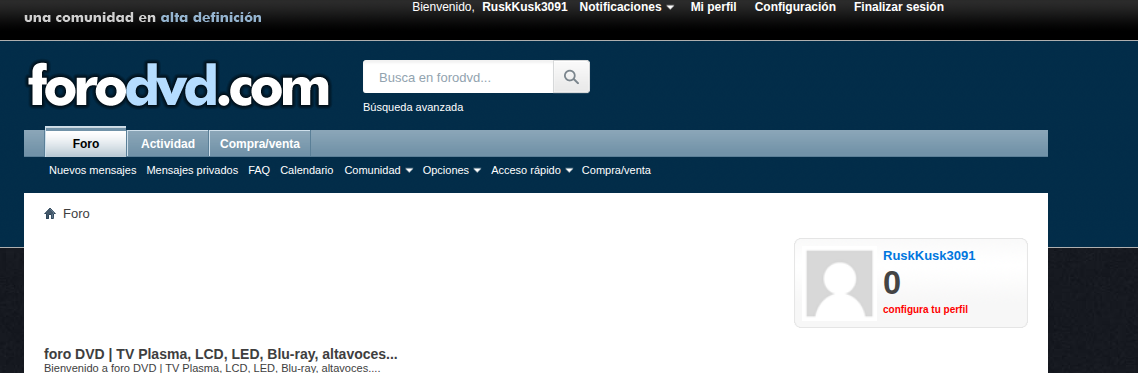
\includegraphics[width=6.5in]{evidencias/E05_control_login_correcto.png}
\par\smallskip
{\small Figura 8. Control previo de acceso con la contraseña correcta.}
\end{minipage}\end{center}
Después de pulsar Forward y desactivar Intercept, ForoDVD mostró el usuario de prueba y la opción Finalizar sesión. La captura siguiente corresponde al resultado de esa solicitud modificada.\par
\begin{center}\begin{minipage}{\linewidth}\centering
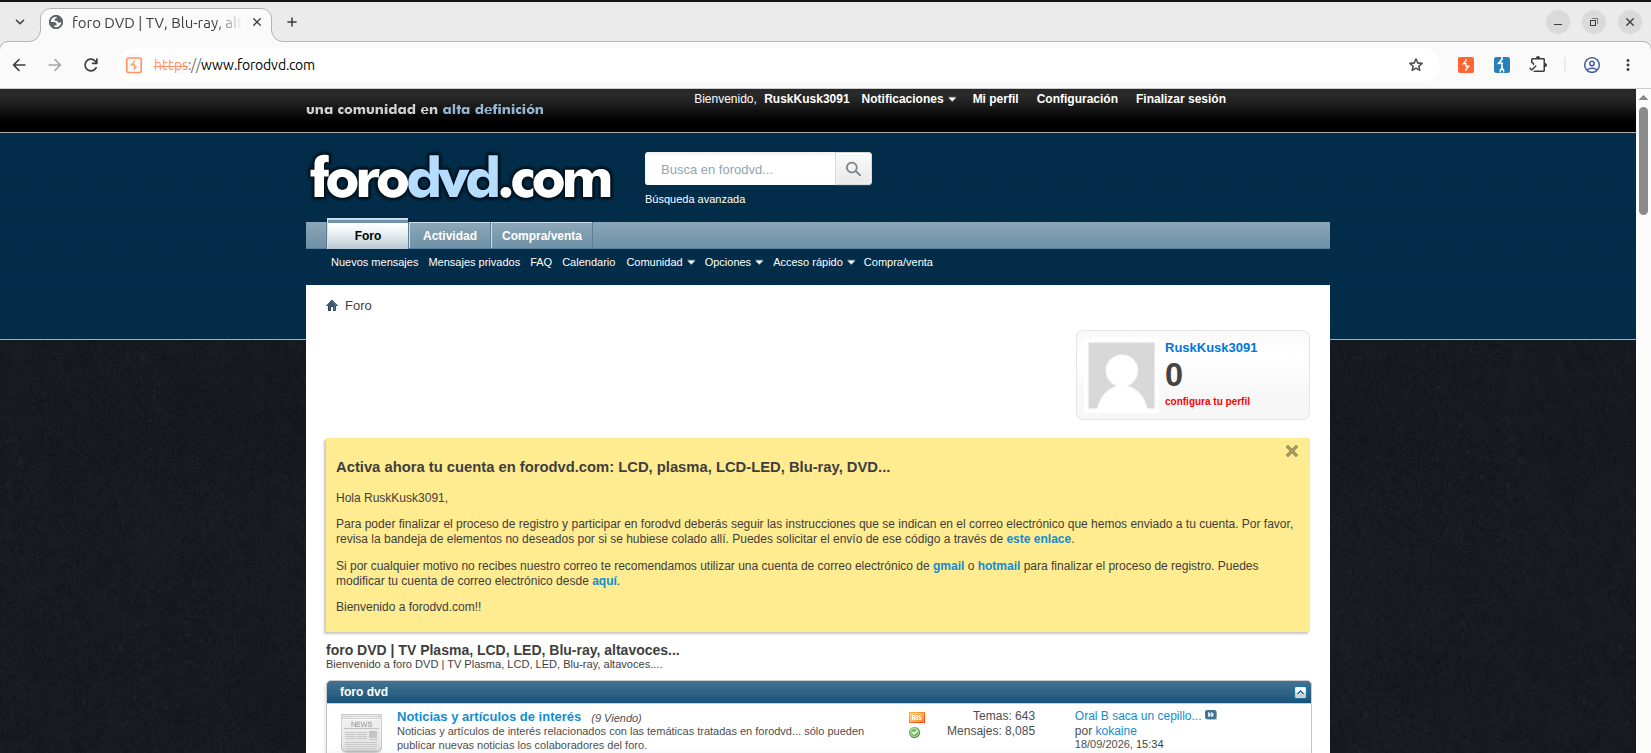
\includegraphics[width=6.5in,trim=225.0314bp 88.5124bp 240.7836bp 66.0092bp,clip]{evidencias/E08_resultado_hash.png}
\par\smallskip
{\small Figura 9. Sesión iniciada después de enviar la solicitud con los hashes sustituidos.}
\end{minipage}\end{center}
El resultado demuestra que, en esta prueba con mi cuenta, el hash capturado fue suficiente para autenticar el acceso al incorporarlo a una solicitud válida. La contraseña escrita inicialmente en el formulario era incorrecta. Se reutilizó el hash como credencial; no fue necesario recuperar la contraseña a partir de ese valor.\par
La cuenta continuó pendiente de activación por correo para participar en el foro. Ese aviso limita la participación y no impidió que el sitio abriera una sesión autenticada.\par
\newpage
\section*{2.6. Identifica las políticas de privacidad o seguridad}
\addcontentsline{toc}{subsection}{2.6. Identifica las políticas de privacidad o seguridad}
El enlace Privacidad del pie de ForoDVD dirige a la política de protección de datos de HD Bits. Revisé ese documento como política publicada por el operador del sitio. [S1, S3]\par
\subsection*{Contenido de la política publicada}
La política identifica a HD Bits Networks SL como responsable del tratamiento. Declara confidencialidad de los datos y reconoce derechos de acceso, rectificación, cancelación y oposición. Indica que una cesión de datos a terceros requeriría informar al usuario y solicitar su consentimiento. También describe comunicaciones comerciales voluntarias y la gestión de preferencias desde el perfil del foro. [S3]\par
La política declara: «Sus datos serán tratados con absoluta confidencialidad». [S3]\par
El texto revisado no detalla el algoritmo usado para las contraseñas, sal, iteraciones, almacenamiento, longitud mínima ni autenticación de varios factores. Por ello, la política aporta compromisos generales sobre datos personales, pero no permite determinar cómo se protegen las contraseñas en el servidor. [S3]\par
Enlace a la política:\\
\url{https://www.hdbits.es/politica-de-proteccion-de-datos/}\par
\subsection*{Controles observados en las pantallas}
{\small\renewcommand{\arraystretch}{1.12}
\begin{longtable}{|>{\raggedright\arraybackslash}p{4.31cm}|>{\raggedright\arraybackslash}p{11.26cm}|}
\hline
\textbf{Control} & \textbf{Evidencia y alcance}\\\hline
\endhead
Contraseña incorrecta & El sitio rechazó el intento sin sustituir el hash.\\\hline
Límite anunciado & Aviso de cinco intentos y bloqueo de 15 minutos; no se agotó el límite.\\\hline
Activación de cuenta & La página pidió activación por correo para participar, aunque permitió iniciar sesión.\\\hline
Cambio de contraseña & El formulario pidió contraseña actual, nueva y confirmación.\\\hline
Mayúsculas y minúsculas & La interfaz indicó que las contraseñas distinguen mayúsculas y minúsculas.\\\hline
\end{longtable}
}
Los controles de esta tabla se identificaron en la ejecución práctica. Se distinguen de las declaraciones de la política para no atribuir al documento detalles que no publica.\par
\newpage
\section*{2.7. Comente 4 conclusiones sobre la seguridad del sitio escogido}
\addcontentsline{toc}{subsection}{2.7. Comente 4 conclusiones sobre la seguridad del sitio escogido}
\subsection*{1 El cliente envía un hash que se mantiene estable}
Para la contraseña de prueba, el registro, la consola y los dos campos del login produjeron el mismo MD5. El cálculo observado no incorporó un reto variable al valor enviado. Esto permitió identificar una credencial derivada estable en las operaciones analizadas. [S2]\par
\subsection*{2 El hash capturado permitió autenticar el acceso}
El acceso con contraseña incorrecta fue rechazado. Al repetir el intento y reemplazar ambos hashes por el valor correcto, el sitio abrió una sesión. Por tanto, quien dispusiera de ese valor y de una solicitud válida podría intentar usarlo como credencial en el contexto probado. El experimento corresponde a la reutilización de hash solicitada por la pauta.\par
\subsection*{3 Los controles adicionales tienen funciones diferentes}
El sitio validó el valor recibido y anunció límites para intentos fallidos. También mantuvo la activación por correo pendiente para participar. En la prueba, estos controles coexistieron con la aceptación del hash correcto reutilizado. El límite de intentos no se evaluó hasta el bloqueo y la activación no se eludió.\par
\subsection*{4 El análisis del cliente tiene un alcance concreto}
Observar MD5 en el navegador y reutilizar ese valor no permite conocer cómo el servidor guarda las contraseñas. La política revisada tampoco publica esos detalles. La conclusión comprobada se limita a la aceptación del hash como credencial en esta cuenta y este flujo. Una evaluación del almacenamiento o de otras cuentas requeriría evidencia adicional. [S3]\par
\section*{Conclusiones y comentarios}
El hash enviado por el cliente debe protegerse como una credencial cuando su posesión permite iniciar sesión. La práctica comprobó este comportamiento mediante el rechazo del control incorrecto, la sustitución de ambos hashes y el acceso posterior con la cuenta propia.\par
En Configuración abrí Editar correo y contraseña, completé la contraseña actual, una nueva y su confirmación, y envié Guardar cambios. El sitio confirmó la actualización del perfil. No volví a probar el hash antiguo después del cambio.\par
\begin{center}\begin{minipage}{\linewidth}\centering
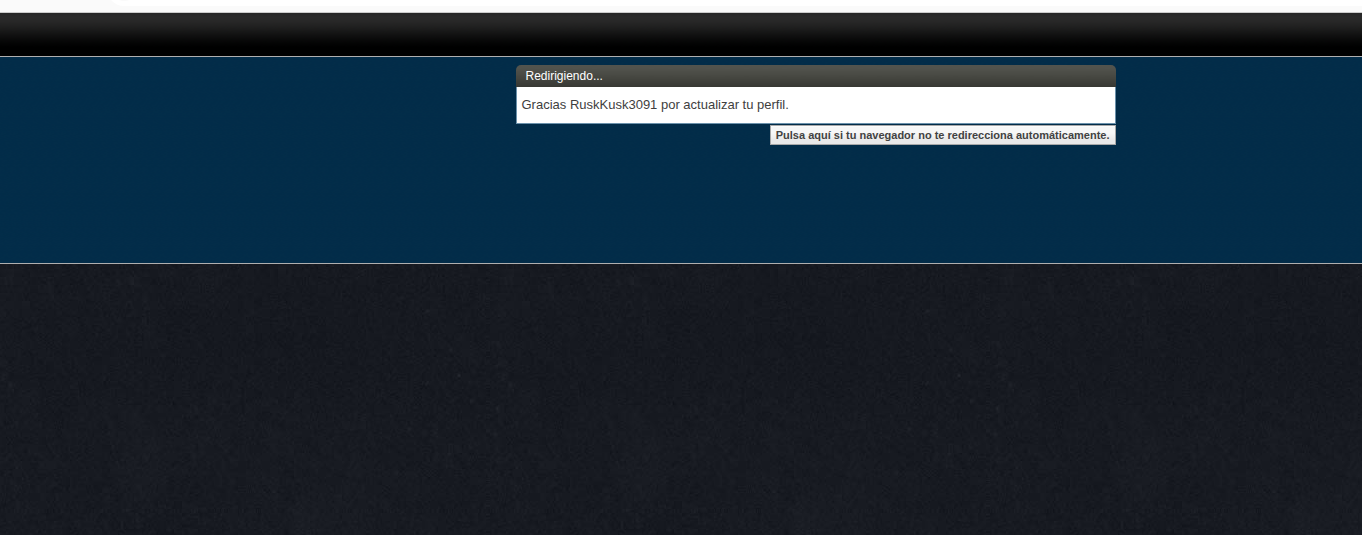
\includegraphics[width=6.5in,trim=378.8029bp 285.0398bp 174.0243bp 41.2558bp,clip]{evidencias/E09_cambio_contrasena.png}
\par\smallskip
{\small Figura 10. Confirmación de actualización después de enviar el cambio de contraseña.}
\end{minipage}\end{center}
\newpage
\section*{Referencias}
Fuentes públicas consultadas el 22 de octubre de 2026. Las capturas corresponden a la cuenta propia de prueba.\par
[S1] ForoDVD registro y formulario público de acceso\\
\url{https://www.forodvd.com/register.php}\par
[S2] ForoDVD biblioteca JavaScript de MD5\\
\url{https://www.forodvd.com/clientscript/vbulletin_md5.js?v=423}\par
[S3] HD Bits política de protección de datos enlazada por ForoDVD\\
\url{https://www.hdbits.es/politica-de-proteccion-de-datos/}\par
[S4] PortSwigger documentación de Proxy Intercept\\
\url{https://portswigger.net/burp/documentation/desktop/tools/proxy/intercept-messages}\par
[S5] PortSwigger modificación de solicitudes con Inspector\\
\url{https://portswigger.net/burp/documentation/desktop/tools/inspector/modify-requests}\par
\subsection*{Evidencias por criterio}
{\small\renewcommand{\arraystretch}{1.12}
\begin{longtable}{|>{\raggedright\arraybackslash}p{3.26cm}|>{\raggedright\arraybackslash}p{1.4cm}|>{\raggedright\arraybackslash}p{10.47cm}|}
\hline
\textbf{Criterio} & \textbf{Puntos} & \textbf{Evidencia disponible}\\\hline
\endhead
2.1 Registro & 5 & Figura 1 y biblioteca pública de MD5.\\\hline
2.2 Login & 5 & Figura 2 y comparación con el registro.\\\hline
2.3 Consola & 15 & Figura 3 con comando y salida reales.\\\hline
2.4 Burp & 10 & Figuras 4 y 5 con solicitud detenida.\\\hline
2.5 Uso del hash & 15 & Figuras 6 a 9 con controles, cambio y resultado.\\\hline
2.6 Políticas & 5 & Enlace, cita breve y análisis del documento.\\\hline
2.7 Conclusiones & 5 & Cuatro conclusiones basadas en la práctica.\\\hline
\end{longtable}
}
La matriz relaciona los siete criterios y sus 60 puntos posibles con las evidencias; la calificación corresponde a la revisión del docente.\par
\section*{Repositorio Git del laboratorio}
\url{https://github.com/rkkas/laboratorio3-forodvd}\par
El repositorio reúne el informe, su fuente LaTeX, las capturas seleccionadas, el comando de consola, el procedimiento, los resultados y la relación con la rúbrica. La procedencia de los recortes se registra en evidencias/\nolinkurl{procedencia_recortes}.json.\par
\end{document}
